% !TEX TS-program = lualatex
\documentclass[11 pt]{amsart}

\usepackage[margin=1.3in]{geometry}

\usepackage{amssymb}
\usepackage{amsmath}
\usepackage{amsthm}
\usepackage{amsfonts}
\usepackage{amsxtra}
\usepackage{bbm}
\usepackage[all,2cell]{xy}
\usepackage{verbatim}
\usepackage{color}
\usepackage{float}
\usepackage{tikz-cd}
\usepackage{multicol}
\usepackage{quiver}
\usepackage{csquotes}
\usepackage[unicode=true, pdfusetitle,
 bookmarks=true,bookmarksnumbered=false,
 breaklinks=false,
 backref=false,
 colorlinks=true,
 linkcolor=blue,
 citecolor=blue,
 urlcolor=blue,
 final
]{hyperref}


\usepackage{bookmark}


\usepackage[capitalise]{cleveref}
\newcommand{\fref}{\cref}
\newcommand{\Fref}{\Cref}
\newcommand{\prettyref}{\cref}
\newcommand{\newrefformat}[2]{}



\theoremstyle{plain}   % This is the default, anyway
\newtheorem{thm}{Theorem}[section] % numbered theorem
\makeatletter\let\c@thm\c@thm\makeatother
\newtheorem{cor}{Corollary}[section]
\makeatletter\let\c@cor\c@thm\makeatother
\newtheorem{lemma}{Lemma}[section]
\makeatletter\let\c@lemma\c@thm\makeatother
\newtheorem{prop}{Proposition}[section]
\makeatletter\let\c@prop\c@thm\makeatother
\newtheorem{claim}{Claim}[section]
\makeatletter\let\c@claim\c@thm\makeatother



\newtheorem*{unnumberedtheorem}{Theorem}  % unnumbered theorem
\newtheorem*{unnumberedcorollary}{Corollary}
\newtheorem*{unnumberedlemma}{Lemma}
\newtheorem*{unnumberedproposition}{Proposition}
\newtheorem*{unnumberedclaim}{Claim}

\theoremstyle{definition}

\newtheorem{defn}{Definition}[section]
\makeatletter\let\c@defn\c@thm\makeatother
\newtheorem{const}{Construction}[section]
\makeatletter\let\c@const\c@thm\makeatother
\newtheorem{notn}{Notation}[section]
\makeatletter\let\c@notn\c@thm\makeatother
\newtheorem{outline}{Proof Outline}[section]
\makeatletter\let\c@outline\c@thm\makeatother


\theoremstyle{remark}

\newtheorem{rem}{Remark}[section]
\makeatletter\let\c@rem\c@thm\makeatother
\newtheorem{ex}{Example}[section]
\makeatletter\let\c@ex\c@thm\makeatother
\newtheorem{observation}{Observation}[section]
\makeatletter\let\c@observationn\c@thm\makeatother

\newtheorem*{unnumberedtheoremremark}{Remark}
\newtheorem*{unnumberedtheoremexample}{Example}
\newtheorem*{unnumberedtheoremdefinition}{Defintion}

\makeatletter
\let\c@equation\c@thm
\numberwithin{equation}{section}
\makeatother


 %Cleveref definitions
\crefname{lemma}{Lemma}{Lemmas}
\crefname{thm}{Theorem}{Theorems}
\crefname{defn}{Definition}{Definitions}
\crefname{notn}{Notation}{Notations}
\crefname{const}{Construction}{Constructions}
\crefname{prop}{Proposition}{Propositions}
\crefname{rem}{Remark}{Remarks}
\crefname{cor}{Corollary}{Corollaries}
\crefname{equation}{Diagram}{Diagrams}
\crefname{ex}{Example}{Examples}



%% ALPHABETS %%
\def\cA{\mathcal{A}}
\def\cB{\mathcal{B}}
\def\cC{\mathcal{C}}
\def\cD{\mathcal{D}}
\def\cE{\mathcal{E}}
\def\cF{\mathcal{F}}
\def\cG{\mathcal{G}}
\def\cH{\mathcal{H}}
\def\cI{\mathcal{I}}
\def\cJ{\mathcal{J}}
\def\cK{\mathcal{K}}
\def\cL{\mathcal{L}}
\def\cM{\mathcal{M}}
\def\cN{\mathcal{N}}
\def\cO{\mathcal{O}}
\def\cP{\mathcal{P}}
\def\cQ{\mathcal{Q}}
\def\cR{\mathcal{R}}
\def\cS{\mathcal{S}}
\def\cT{\mathcal{T}}
\def\cU{\mathcal{U}}
\def\cV{\mathcal{V}}
\def\cW{\mathcal{W}}
\def\cX{\mathcal{X}}
\def\cY{\mathcal{Y}}
\def\cZ{\mathcal{Z}}

\def\AA{\mathbb{A}}
\def\BB{\mathbb{B}}
\def\CC{\mathbb{C}}
\def\DD{\mathbb{D}}
\def\EE{\mathbb{E}}
\def\FF{\mathbb{F}}
\def\GG{\mathbb{G}}
\def\HH{\mathbb{H}}
\def\II{\mathbb{I}}
\def\JJ{\mathbb{J}}
\def\KK{\mathbb{K}}
\def\LL{\mathbb{L}}
\def\MM{\mathbb{M}}
\def\NN{\mathbb{N}}
\def\OO{\mathbb{O}}
\def\PP{\mathbb{P}}
\def\QQ{\mathbb{Q}}
\def\RR{\mathbb{R}}
\def\SS{\mathbb{S}}
\def\TT{\mathbb{T}}
\def\UU{\mathbb{U}}
\def\VV{\mathbb{V}}
\def\WW{\mathbb{W}}
\def\XX{\mathbb{X}}
\def\YY{\mathbb{Y}}
\def\ZZ{\mathbb{Z}}

%% OTHER SYMBOLS %% 
\DeclareMathOperator{\id}{id}
\DeclareMathOperator{\dom}{dom}
\DeclareMathOperator{\cod}{cod}

\def\nat{\Rightarrow}
\def\monic{\rightarrowtail}
\def\epic{\twoheadrightarrow}
\def\pathto{\rightsquigarrow}
\def\Aut{\text{Aut}}

\newcommand{\punctuation}[1]{\makebox[0pt][l]{#1}}
\newcommand{\cat}[1]{{\normalfont\texttt{#1}}}
\newcommand{\op}[1]{{{#1}^{\cat{op}}}}
\newcommand{\opc}[1]{\op{\cat{#1}}}
\newcommand{\Obj}[1]{\text{Obj}(\cat{#1})}
\newcommand{\Map}[1]{\text{Map}(\cat{#1})}

% https://tex.stackexchange.com/a/118217
% \DeclarePairedDelimiter\ceil{\lceil}{\rceil}
% \DeclarePairedDelimiter\floor{\lfloor}{\rfloor}

\title{The Fundamental Groupoid}

\author{Riley Shahar}

\pagestyle{plain}

\parindent0pt
\parskip4pt


\begin{document}



\begin{abstract}
	We introduce basic category theory and construct the fundamental groupoid of a
	topological space. Using homotopy as an analogy, we define natural
	transformations and equivalence of categories. We conclude with the
	homotopy invariance of the fundamental groupoid and a sketch of strict
	2-categories.
\end{abstract}


\maketitle

\section{Introduction}

The fundamental groupoid is a generalization of the better-known fundamental
group which captures information of the entire space, instead of just a single
basepoint. It naturally emerges when one considers generalizing the
categorification of a group. However, the fundamental groupoid is in some sense
not a strict homotopy invariant: the disk and the point have non-isomorphic
fundamental groupoids!

Instead, the correct notion of equivalence on groupoids relies on a notion
called equivalence of categories. The line of thinking which leads to this
definition draws heavy analogies between topological spaces and categories.
Equivalence of categories turns out to be closely related to the familiar notion
of homotopy equivalence. These connections are made rigorous by higher category
theory.

After introducing some basic category theory in \Cref{categories}, we construct
the fundamental groupoid in \Cref{the fundamental groupoid}. This motivates
natural transformations in \Cref{natural transformations}, culminating in a
proof of the homotopy invariance of the fundamental groupoid. We conclude in
\Cref{2 categories} with a brief discussion of 2-categories.

\section{Categorical Preliminaries}\label{categories}

Many of the constructions we'll encounter are categorical, or at least are
well-stated using categorical ideas, so it's worth spending some time with basic
category theory. Our aim will be to develop only some essential language now,
and later use our exploration of homotopy as motivation for developing higher
category theory. Except where noted, I follow \cite[Sections 1.1-1.3]{Riehl}.

\subsection{Categories}

\begin{defn}
	A \emph{category} $\cat{C}$ consists of a collection of \emph{objects} $\Obj{C}$
	and a collection of \emph{morphisms} $\Map{C}$, such that

	\begin{itemize}
		\item Each morphism $f$ has a specific \emph{domain} $\dom(f)$ and
		      \emph{codomain} $\cod(f)$; we write $f: x\rightarrow y$ or
		      $x\xrightarrow{f} y$.
		\item Each object $x$ has a specific \emph{identity morphism} $1_x:
			      x\rightarrow x$.
		\item For each pair of morphisms $x\xrightarrow{f} y\xrightarrow{g}
			      z$, there is a specific \emph{composite morphism} $gf:
			      x\rightarrow z$. We call $f$ and $g$ \emph{composition-compatible}.
	\end{itemize}
	This data must be \emph{associative} and \emph{unital}, which is to say,
	\begin{itemize}
		\item (Associativity) For each composition-compatible triplet, i.e.
		      $x\xrightarrow{f}y \xrightarrow{g}z\xrightarrow{h}w$, we have $h(gf) =
			      (hg)f$. We write merely $hgf$.
		\item (Unital) For any $f: x\rightarrow y$, we have $1_yf = f = f1_x$.
	\end{itemize}

	In other words, the following diagrams commute:

	\begin{figure}[H]
		\centering
		\begin{multicols}{2}
			\begin{tikzcd}
				x & y & z & w
				\arrow["f", from=1-1, to=1-2]
				\arrow["g", from=1-2, to=1-3]
				\arrow["h", from=1-3, to=1-4]
				\arrow["gf"', curve={height=18pt}, from=1-1, to=1-3]
				\arrow["hg", curve={height=-18pt}, from=1-2, to=1-4]
			\end{tikzcd}

			\begin{tikzcd}
				x & x \\
				& y
				\arrow["1_x", from=1-1, to=1-2]
				\arrow["f", from=1-2, to=2-2]
				\arrow["f"', from=1-1, to=2-2]
			\end{tikzcd}
			\begin{tikzcd}
				x & y \\
				& y
				\arrow["f", from=1-1, to=1-2]
				\arrow["1_y", from=1-2, to=2-2]
				\arrow["f"', from=1-1, to=2-2]
				\punctuation{.}
			\end{tikzcd}
		\end{multicols}
	\end{figure}
\end{defn}


\begin{notn} We will use $\cat{C}(x, y)$ for the morphisms with domain $X$ and
	codomain $Y$. We also choose to use multiplicative notation for composition,
	instead of $\circ$, to distinguish it from function composition, since in many
	of our categories morphism composition will be concatenation or something
	completely separate from function composition. \end{notn}

\begin{ex}\label{concrete categories} Many mathematical structures can be studied as categories:
	\begin{itemize}
		\item $\cat{Set}$ is the category of sets and set-functions.
		\item $\cat{Poset}$ is the category of partially ordered sets and
		      monotone functions.
		\item $\cat{Grp}$ is the category of groups and homomorphisms.
		\item $\cat{Top}$ is the category of topological spaces and continuous
		      functions.
		\item For any field $\Bbbk$, $\cat{Vect}_\Bbbk$ is the category of vector
		      spaces over $\Bbbk$ and linear maps.
	\end{itemize}
\end{ex}

These examples demonstrate the need for the word ``collection'' in the
definition of a category: there is no set of all sets, for example. In general,
we'll avoid detailing the set-theoretic issues here.

\begin{defn} A category is \emph{small} when its morphisms
	form a set. A category is \emph{locally small} when, for each pair of objects $x,
		y$, the morphisms $\cat{C}(x, y)$ forms a set. \end{defn}

\begin{rem}
	Any small category is locally small, since the morphisms between two objects
	form a subset of the set of morphisms. The objects in any small category form
	a set, since they are in bijection with the identity morphisms, which form a
	subset of the set of morphisms.
\end{rem}

None of the categories in \Cref{concrete categories} is small. In fact, each of
these examples takes as objects sets with certain structure and as morphisms
structure-preserving functions between those sets. As the following example
shows, these are far from the only kind of category.

\begin{ex}\label{abstract categories} The following are also categories:
	\begin{itemize}
		\item The \emph{empty category} is the category with no objects and no
		      morphisms.
		\item The \emph{trivial category} is the category with one object and only
		      its identity morphism.
		\item A set $X$ can be represented as a category whose objects correspond
		      with the elements of $X$ and which has only identity morphisms. A category
		      with only identity morphisms is called \emph{discrete}.
		\item A group $G$ can be represented as a category with one object whose
		      morphisms correspond with the element of $G$, with composition
		      determined by multiplication. Following \cite{Porter}, we call this
		      category $\GG$.
		\item A poset $P$ can be represented as a category whose objects correspond
		      with the elements of $P$ and with a single morphism $x\rightarrow y$
		      whenever $x\leq y$. We call this category $\PP$.
	\end{itemize}
\end{ex}

\subsection{(Iso)morphisms}

The main philosophy of category theory is roughly that

\begin{displayquote}
	an object is completely determined by its relationship with other objects,
	\cite[p. 8]{Bradley}
\end{displayquote}

and so to study an object, one should study its morphisms. I can't resist
sharing the following example:

\begin{ex}\cite[Example 2.1.6(ii)]{Riehl}
	Fixing a topological space $X$, we can recover both the points of $X$ and the
	topology on $X$---in other words, all the data of the space---via studying
	only maps involving $X$, as follows.

	To recover the points, note that a map $f: *\rightarrow X$, where $*$ is the
	singleton space, consists of picking out any point $f(*)\in X$. Thus the
	points are in bijection with $\cat{Top}(*, X)$.

	To recover the topology, let $S = \{0, 1\}$ with the topology $\{\emptyset,
		\{1\}, X\}$. To any open set $U\subseteq X$, associate the map
	$$f_U(x) = \begin{cases}
			1 & \text{ if }x\in U    \\
			0 & \text{ if }x\notin U
		\end{cases}$$

	But we can write any continuous function $f: X\rightarrow S$ in this form by
	setting $U = f^{-1}(\{1\})$. Thus the open sets are in bijection with
	$\cat{Top}(X, S)$.
\end{ex}

A chiefly important kind of morphism is the \emph{isomorphism}, which (as in
most algebraic contexts) suggests a fundamental similarity between its domain and
codomain.

\begin{defn}
	A morphism $f: x\rightarrow y$ is an \emph{isomorphism} when there is a morphism
	$g: y\rightarrow x$ such that $gf = 1_x$ and $fg = 1_y$. We call $g$ the
	\emph{inverse} of $f$ and write $g = f^{-1}$. We say $x$ and $y$ are
	\emph{isomorphic} and write $x\cong y$.
\end{defn}

\begin{ex}\label{isomorphisms} Isomorphisms are interesting in many of our examples of categories:
	\begin{itemize}
		\item In $\cat{Set}$, the isomorphisms are invertible set-functions, i.e. bijections.
		\item In $\cat{Grp}$, the isomorphisms are group isomorphisms.
		\item In $\cat{Top}$, the isomorphisms are homeomorphisms.
		\item In $\cat{Vect}_{\Bbbk}$, the isomorphisms are vector space isomorphisms.
		\item For any group $G$, any morphism in $\GG$ is an isomorphism;
		      this fact corresponds to the existence of inverses in the group. (We
		      will have more to say about this example in \Cref{sec:groupoids}.)
		\item For any poset $P$, the isomorphisms in $\PP$ are the identities;
		      this fact corresponds to anti-symmetry of the relation.
	\end{itemize}
\end{ex}

\begin{lemma}\label{inverses are unique}
	Let $f: x\rightarrow y$ be an isomorphism with inverses $g$ and $h$. Then $g = h$.
\end{lemma}

\begin{proof}
	We have $g = 1_xg = (hf)g = h(fg) = h1_y = h.$
\end{proof}

\begin{notn}
	\Cref{inverses are unique} justifies writing the inverse of an isomorphism $f$
	as $f^{-1}$, since it guarantees this specifies a unique morphism.
\end{notn}

Further, as we expect:

\begin{prop}\label{isomorphism is equivalence}
	Isomorphism forms an equivalence relation on the class of objects in
	a category $\cat{C}$.
\end{prop}

\begin{proof} We need to show:
	\begin{itemize}
		\item Reflexivity. The identity $1_x$ is an isomorphism $x\rightarrow x$.
		\item Symmetry. For $f: x\rightarrow y$ an isomorphism, $f^{-1}$ is an
		      isomorphism $y\rightarrow x$, with inverse $f$.
		\item Transitivity. For $f: x\rightarrow y$ and $g: y\rightarrow z$
		      isomorphisms, $gf$ is an isomorphism $x\rightarrow z$, with inverse
		      $f^{-1}g^{-1}$. \qedhere
	\end{itemize}
\end{proof}

In a locally small category $\cat{C}$, where $f: x\rightarrow y$ is any morphism
and $z$ is an ambient object, we can define maps $f_*: \cat{C}(z, x)\rightarrow
	\cat{C}(z, y)$ and $f^*: \cat{C}(y, z)\rightarrow \cat{C}(x, z)$ via post- and
pre-composition by $f$, respectively. In this case, \Cref{isomorphism
	characterization} gives an important characterization of isomorphisms in terms
of these maps.

\begin{thm}\label{isomorphism characterization}Let $\cat{C}$ be locally small.
	Then the following are equivalent:

	\begin{enumerate}
		\item  $f: x\rightarrow y$ is an isomorphism.
		\item  For every $z\in\cat{C}$, $f_*$ is a bijection of sets.
		\item For every $z\in\cat{C}$, $f^*$ is a bijection of sets.
	\end{enumerate}
\end{thm}

\begin{rem}
	If objects are characterized by their morphisms, then \Cref{isomorphism
		characterization} supports the idea that isomorphic objects truly look the
	same to the machinery of the category.
\end{rem}

\begin{proof}[Proof of \Cref{isomorphism characterization}]
	We prove equivalence $(1)\Leftrightarrow(2)$; the proof $(1)\Leftrightarrow(3)$ is
	similar\footnote{One can also conclude the latter via studying $(2)$ in the
		context of the \emph{opposite category} of $\cat{C}$, but this is outside our
		scope. See \cite[Lemma 1.2.3]{Riehl} for such a proof.}.

	Let $f$ be an isomorphism. We show $f^{-1}_*$ is an inverse of
	$f_*$. In particular, for any morphisms $h: z\rightarrow x$ and $k:
		z\rightarrow y$, we have that
	$$f^{-1}_*(f_*(h)) = f^{-1}fh = 1_Xh = h
		\quad
		\text{ and }
		\quad
		f_*(f^{-1}_*(k)) = ff^{-1}k = 1_Yk = k.$$

	Conversely, let $f_*$ be bijective. Letting $z = y$, by surjectivity there is
	some $g\in\cat{C}(y, x)$ such that $1_y = f_*(g) = fg$. But now letting $z =
		x$, we see that $$f_*(gf) = fgf = 1_yf = f = f_*(1_x),$$ and so by injectivity
	$gf = 1_x$. Thus $g$ is an inverse of $f$, hence $f$ is an isomorphism.
	\qedhere

\end{proof}

\subsection{Functors}

If the philosophy of category theory is to study morphisms between objects, then
functors answer the obvious question: what are the morphisms between categories?

\begin{defn}
	A \emph{functor} $F: \cat{C}\rightarrow\cat{D}$ between
	categories $\cat{C}$ and $\cat{D}$ consists of
	\begin{itemize}
		\item For each object $x\in\Obj{C}$, an object $Fx\in\Obj{D}$.
		\item For each morphism $f\in\Map{C}$, a morphism $Ff\in\Map{D}$.
	\end{itemize}

	This data must preserve the categorical structure, i.e. domains, codomains,
	identities, and composites, that is,

	\begin{itemize}
		\item For each $f\in\Map{C}$, $\dom(Ff) = F(\dom(f))$ and $\cod(Ff) =
			      F(\cod(f))$.
		\item For each composition-compatible pair $f,g\in\Map{C}$, $(Fg)(Ff) =
			      F(gf)$.
		\item For each $x\in\Obj{C}$, $F(1_x) = 1_{Fx}$.
	\end{itemize}
\end{defn}

\begin{ex}\label{functors}
	Many common constructions are functors:
	\begin{itemize}
		\item On any category $\cat{C}$ there is an \emph{identity functor}
		      $1_\cat{C}$.
		\item The power set defines a functor $\cP:
			      \cat{Set}\rightarrow\cat{Set}$ which takes a morphism $f$ to its
		      action via images, i.e. $\cP(f)(A) = f(A)$.
		\item On a category $\cat{C}$ like those in \Cref{concrete categories}, the
		      \emph{forgetful functor} $\cat{C}\rightarrow\cat{Set}$ sends an object to
		      its underlying set and a morphism to its underlying set-function,
		      ``forgetting'' the algebraic structure.
		\item The free group defines a functor $\cat{Set}\rightarrow\cat{Grp}$ which
		      sends a set to its free group and a map to its letter-wise action on
		      words.
		\item A group action of a group $G$ on a set $A$ can be regarded as a functor
		      $\GG\rightarrow\cat{Set}$ which sends the single object of $\GG$ to $A$ and
		      a morphism to the endofunction defined by that element's action on
		      $A$. In fact, the funtoriality axioms correspond precisely to the
		      axioms of group action.
		\item The construction $f_*$ from \Cref{isomorphism characterization} gives
		      a functor $\cat{C}(z, -): \cat{C}\rightarrow\cat{Set},$ called the
		      \emph{covariant functor represented by $z$}, which sends any object $x$ to
		      $\cat{C}(z, x)$\footnote{The analogous functor for $f^*$ requires a
			      little more machinery in the form of \emph{contravariant functors}, outside
			      our scope. These representation functors are critically important
			      for tools central category-theoretic tools such as \emph{universal
				      properties} and the \emph{Yoneda lemma}. See \cite[Chapter 2]{Riehl}.}.
	\end{itemize}
\end{ex}

\begin{thm}\label{functors preserve isomorphism}
	Let $F: \cat{C}\rightarrow \cat{D}$ be a functor and $f: x\rightarrow y$ an isomorphism in
	$\cat{D}$. Then $Ff$ is an isomorphism between $Fx$ and $Fy$ in $\cat{D}$.
\end{thm}

\begin{proof}
	We have $$(Ff^{-1})(Ff) = F(f^{-1}f) = F1_x = 1_{Fx},$$
	and the same works on the other side.
\end{proof}

There is a category of categories, $\cat{Cat}$, whose objects are categories and
whose morphisms are functors\footnote{Categories in \cat{Cat} must be locally
	small, for set-theoretic reasons. It is common, e.g. in \cite{Riehl}, to call
	this category $\cat{CAT}$, to distinguish it from the category of small
	categories, which in turn is called $\cat{Cat}$. As we ignore these details, we
	use the more convenient notation.}. Composition of functors is defined in the
obvious way. This allows us to define isomorphic categories straightforwardly:

\begin{defn}
	Two categories $\cat{C}$ and $\cat{D}$ are \emph{isomorphic} when there is a
	functor $F: \cat{C}\rightarrow\cat{D}$ which is an isomorphism in $\cat{Cat}$.
\end{defn}

We will see later, in \Cref{fundamental groupoid is not homotopy invariant}, that
this definition is generally too restrictive. That will motivate our discussion of
\emph{natural transformations} in \Cref{natural transformations}, where we will
define a more useful notion of \emph{equivalence of categories}. One hint at the
restrictiveness is the following:

\begin{thm}\label{isomorphisms are bijections}\cite[Theorem 6.4.3]{Brown}
	A functor $F: \cat{C}\rightarrow\cat{D}$ between small categories is an
	isomorphism if and only if it is a bijection on both objects and
	morphisms.
\end{thm}

\begin{proof}
	Let $F$ be an isomorphism with inverse $G$. For any $x\in\Obj{C}$, $(GF)x =
		1_\cat{C}x = x$; this shows $F$ is invertible, hence bijective, as a function
	on $\Obj{C}$. The same works for morphisms.

	Conversely, let $F$ be a bijection on both objects and morphisms, with inverse
	$G$. We need to check that $G$ is a functor and an inverse of $F$. The latter
	is easy, since it is an inverse on both objects and morphisms.

	To check functoriality, it suffices to check images of $F$, by surjectivity.
	\begin{itemize}
		\item Let $x\in\Obj{C}$. By functoriality of $F$, $G1_{Fx} = 1_x$.
		\item Let $f,g\in\Map{C}$ be composition-compatible. Then $$G(FgFf) = G(Fgf)
			      = gf = GFg\cdot GFf,$$ as desired. \qedhere
	\end{itemize}
\end{proof}

\subsection{Groupoids}\label{sec:groupoids}

According to \Cref{abstract categories} and \Cref{isomorphisms}, any group can
be represented by a specific kind of category, one with a single object and only
isomorphisms. Indeed, any such category assembles into a group:

\begin{itemize}
	\item Elements are given by morphisms, with multiplication given by
	      composition.
	\item Multiplication is well-defined because any two morphisms have the same
	      domain and codomain (the single object), and hence are
	      composition-compatible.
	\item Multiplication is associative because composition is associative.
	\item The group identity is the identity morphism on the single object.
	\item Morphisms have inverses since they are isomorphisms.
\end{itemize}

It turns out that the requirement of a single object isn't necessary for the
algebraic structure we recover to be interesting. Indeed, relaxing this
requirement gives our fundamental object of study:

\begin{defn}
	A \emph{groupoid} is a category in which every morphism is an isomorphism.
\end{defn}

The second bullet above suggests that a groupoid will have to sacrifice
well-definideness of multiplication. Indeed, there is a purely algebraic picture
of groupoids defined in terms of partial functions, but the categorical one will
be sufficient for our needs. For a more complete discussion, see \cite{Brown}.

\begin{defn}\label{groupoids}
	We can define several common kinds of groupoids:
	\begin{itemize}
		\item A groupoid with one element is a \emph{group}. Per the above
		      discussion, we can indeed take this as a definition.
		\item A groupoid with only identity morphisms is a \emph{discrete groupoid}.
		      Such groupoids correspond bijectively to sets; see \Cref{concrete categories}.
		\item A groupoid with at least one morphism between any two objects is \emph{connected}.
		\item A groupoid with precisely one morphism between any two objects is a
		      \emph{tree groupoid}.
	\end{itemize}
\end{defn}

Since groupoids are defined as categories, the morphisms between them are
functors:

\begin{defn}\cite[Section 6.4]{Brown}
	A \emph{groupoid morphism} is a functor between groupoids.
\end{defn}

Unsurprisingly, there is a category, $\cat{Grpd}$, of groupoids and groupoid
morphisms.

\section{The Fundamental Groupoid} \label{the fundamental groupoid}

A central idea of algebraic topology is that topological notions are encoded in
algebraic invariants of a space. The first such invariant we study is the
\emph{fundamental groupoid}, in some sense a more natural object than the
fundamental group, constructed from the homotopy classes of paths in a space.
Except where noted, I follow \cite[Chapter 6]{Bradley}.

\subsection{Homotopy}\label{sec:homotopy}

Recall that a \emph{homotopy} between continuous functions $f,g: X\rightarrow Y$
is a continuous function $H: X\times I\rightarrow Y$ such that $H(-, 0) = f$ and
$H(-, 1) = g$; in other words, the following diagram commutes:

\begin{figure}[H]
	\centering
	\begin{tikzcd}
		X & X\times I & X \\
		& Y\punctuation{,} &
		\arrow["i_0", from=1-1, to=1-2]
		\arrow["i_1", from=1-3, to=1-2, swap]
		\arrow["f", from=1-1, to=2-2, swap]
		\arrow["g", from=1-3, to=2-2]
		\arrow["H", from=1-2, to=2-2]
	\end{tikzcd}
\end{figure}

where $i_0$ and $i_1$ are the inclusions at $(-, 0)$ and $(-, 1)$.

This homotopy is further a \emph{path homotopy}\footnote{ When
	the context is unclear, we will call a general homotopy a \emph{free
		homotopy}, and a homotopy with fixed endpoints a \emph{path homotopy}. } when $X
	= I$ (so $f$ and $g$ are paths) and when $H(0, -)$ and $H(1, -)$ are constant.

Two functions are \emph{homotopic} when there exists a homotopy between them. We
write $f\simeq g$. When the functions are paths and the homotopy is a path
homotopy, the paths are \emph{path homotopic} and we write $f\simeq_p g$. Both
are equivalence relations on the class of functions with appropriate domain and
codomain.

Two spaces $X$ and $Y$ are \emph{homotopy equivalent} when there are maps $f:
	X\rightarrow Y$ and $g: Y\rightarrow X$ such that $fg\simeq 1_Y$ and $gf\simeq
	1_X$. This is an equivalence relation on the spaces; we write $X\simeq Y$.

We can form the category $\cat{hTop}$ by taking spaces as objects and homotopy
classes of maps as morphisms. One needs to check that composition is
well-defined in this category; this was done in class.

\begin{rem} Two spaces are homotopy equivalent precisely they are isomorphic in
	$\cat{hTop}$. There is a functor $\cat{Top}\rightarrow\cat{hTop}$ that is the
	identity on objects and sends a continuous function to its path homotopy
	class. We therefore call functors out of $\cat{hTop}$ \emph{homotopy
		invariants}, since by \Cref{functors preserve isomorphism} they homotopy
	equivalent spaces to isomorphic objects. \end{rem}

\subsection{Construction}

Before defining the fundamental groupoid, there is a nice geometric intuition. Fix
a topological space $X$ and pick some points and paths between those points.
When you ``erase'' the other information of the underlying space, you get
several points and a bunch of (double-headed) arrows.

\begin{figure}[H]
	\centering
	\usetikzlibrary{decorations.markings}

\newcommand{\pathA}{(2, 2) .. controls (3,2) and (3, 1.5) .. (4, 1.5)}
\newcommand{\pathB}{(4, 1.5) .. controls (5, 1.5) and (5,2) .. (6, 2)}
\newcommand{\pathC}{(6, -2) .. controls (5,-2) and (5, -1.5) .. (4, -1.5)}
\newcommand{\pathD}{(4, -1.5) .. controls (3, -1.5) and (3,-2) .. (2, -2)}

\begin{tikzpicture}
	% outer shape
	\filldraw[fill=black, fill opacity=0.2, draw=black] (0, 0) arc(180:90:2) --
	\pathA --
	\pathB --
	(6, 2) arc(90:0:2) --
	(8, 0) arc(360:270:2) --
	\pathC --
	\pathD --
	(2, -2) arc(270:180:2)
	;

	% inner holes
	\filldraw [fill=white] (2,0) circle (1);
	\filldraw [fill=white] (6,0) circle (1);

	% paths
	\coordinate (x) at (3.4, 0.6);
	\node [circle, fill, inner sep=2pt] at (x) {};
	\draw[<->] ([shift=(37:1.5)]2,0) arc(37:370:1.5);
	\draw[<-] (3.65, 0.8) .. controls (4,1) and (5,1.5) .. (6, 1.5);
	\draw[<-] (3.7, 0.4) .. controls (4.5,0) and (5,-1.5) .. (6, -1.5);
	\draw ([shift=(270:1.5)]6,0) arc(270:450:1.5);

	\coordinate (x) at (12.4, 0.6);
	\node [circle, fill, inner sep=2pt] at (x) {};
	\draw[<->] ([shift=(37:1.5)]11,0) arc(37:370:1.5);
	\draw[<-] (12.65, 0.8) .. controls (13,1) and (14,1.5) .. (15, 1.5);
	\draw[<-] (12.7, 0.4) .. controls (13.5,0) and (14,-1.5) .. (15, -1.5);
	\draw ([shift=(270:1.5)]15,0) arc(270:450:1.5);
\end{tikzpicture}
% \begin{tikzpicture}[>={[inset=0,angle'=27]Stealth}]
% 	\draw circle(2);
% 	\draw [thick,fill=cyan!20](230:2)--(0,0)--(130:2) arc (130:230:2)--cycle;
% 	\draw [->](0,0)--node[above]{$r$} (10:2);
% 	\draw [|<->|](130:2.3) arc (130:230:2.3) node[left,pos=.5]{$L$};
% 	\draw [<->]  (130:1)   arc (130:230:1)   node[left,pos=.5]{$\theta$};
% \end{tikzpicture}
% \begin{tikzpicture}
% 	\draw (0,0) .. controls (1,1) and (2,-1) .. (0,0);
% 	% \begin{scope}[transparency group, opacity=0.6]
% 	% 	\path [draw=none, fill=gray] (-1.5,0) circle (2);
% 	% 	\path [draw=none, fill=gray] (1.5,0) circle (2);
% 	% \end{scope}
% \end{tikzpicture}

	\caption{Some points and paths on a two-holed disk.}
	\label{fig:group}
\end{figure}

This looks suspiciously like a groupoid---in particular, each of the arrows are
double-headed, and hence ``invertible''. The issue is that we don't necessarily
see the inverses or composites when we just take some points and some paths.

We'll return to this intuition of the fundamental groupoid ``forgetting'' some of
the underlying geometry of the space. More immediately, however, this view
strongly suggests that when we take all the path classes from our underlying space,
we should get back a groupoid.

\begin{defn}
	The \emph{fundamental groupoid} $\Pi_1X$ of a space $X$ is the category
	whose objects are the points of $X$ and whose morphisms are the path homotopy
	classes of paths in $X$.
\end{defn}

Specifically, let $x,y,z\in X$, $f$ a path from $x$ to $y$, and $g$ a path from
$y$ to $z$. Then,

\begin{itemize}
	\item A path's domain is its startpoint: $\dom([f]) = x$.
	\item A path's codomain is its endpoint: $\cod([f]) = y$.
	\item The identity is the constant map: $1_x = [c_x]$.
	\item Composition is concatenation: $[g][f] = [f*g]$.
\end{itemize}

This construction is well-defined specifically because we are working with path
homotopies. For example, in general two paths with different start points may be
free homotopic, meaning without restricting to path homotopy we could not even
write down the domain and codomain of our morphisms.

\begin{ex}\cite[p. 213]{Brown}
	We can immediately compute a few fundamental groupoids.
	\begin{itemize}
		\item The fundamental groupoid of a convex subspace of $\RR^n$ is a tree
		      groupoid (see \Cref{groupoids}). This corresponds to the fact that
		      any two paths with the same endpoints in such a space are homotopic via
		      the straight line homotopy.
		\item The fundamental groupoid of a totally disconnected space is a discrete
		      groupoid. This corresponds to the fact that the only paths in such spaces
		      are the constant paths.
	\end{itemize}
\end{ex}

\subsection{Categorical Properties} We can learn a lot about the fundamental
groupoid by studying it categorically. First, we should confirm it is what we
claim it is:

\begin{prop}\label{fundamental groupoid is a groupoid}
	The fundamental groupoid is a groupoid.
\end{prop}

\begin{proof}
	All of this work was already done in class for the fundamental group. We
	restate the results here for groupoids.
	\begin{itemize}
		\item Composition is well-defined, since concatenation preserves homotopy
		      class.
		\item Composition is associative, since concatenation is associative up to
		      homotopy.
		\item Every object $x$ has $[c_x]$ as an identity, where $c_x$ is the
		      constant path at $x$.
		\item Every morphism $[f]$ has $[\bar{f}]$ as an inverse, where $\bar{f}$ is
		      $f$ traversed in reverse.
	\end{itemize}

	The first three say that $\Pi_1X$ is a category, and the last says that it
	is a groupoid.
\end{proof}

The construction of the fundamental groupoid naturally gives rise to a functor
$$\Pi_1: \cat{Top}\rightarrow\cat{Grpd}.$$ In particular, let $f: X\rightarrow
	Y$ be a continuous function. We can view $f$ as acting on paths via composition.
Accordingly, we define
\begin{align*}
	\Pi_1f  \colon \Pi_1X & \to \Pi_1Y              \\
	[\gamma]              & \mapsto [f\circ\gamma].
\end{align*}

This mapping is well-defined because composition preserves homotopy equivalence.

\begin{prop}\label{fundamental groupoid is a functor}
	The fundamental groupoid is a functor.
\end{prop}

\begin{proof}
	Let $X\xrightarrow{f}Y\xrightarrow{g}Z$ be spaces and continuous maps. Let
	$\gamma$ be a path in $X$.

	We have $$\Pi_1g\Pi_1f([\gamma]) = \Pi_1g([f\circ\gamma]) = [g\circ f\circ\gamma] = \Pi_1(gf)[\gamma]$$
	and $$\Pi_11_X([\gamma]) = [1_X\circ\gamma] = [\gamma] = 1_{\Pi_1X}([\gamma]).$$
	Thus $\Pi_1$ is compatible with composition and identities, as desired.\qedhere
\end{proof}

This result is an improvement over the fundamental group, where we needed a
functor out of based spaces for the definition to make sense. This is a first
hint that the fundamental groupoid in some sense captures more of the structure
of a space than the fundamental group does.

\begin{cor}\label{fundamental groupoid is topological}
	The fundamental groupoid is a topological invariant. More precisely, if
	$X\cong Y$, then $\Pi_1X\cong \Pi_1Y$.
\end{cor}

\begin{proof}
	This follows from \Cref{functors preserve isomorphism} and \Cref{fundamental
		groupoid is a functor}.
\end{proof}

\begin{rem}\label{fundamental groupoid is not homotopy invariant} As defined,
	the fundamental groupoid is a \emph{not} a homotopy invariant. For instance,
	since objects of the fundamental groupoid are in bijection with elements of
	the underlying space, the fundamental groupoid of $D^n$ has uncountably many
	objects, whereas the fundamental groupoid of the point has only one, hence
	they are not isomorphic by \Cref{isomorphisms are bijections}; nevertheless,
	$D^n$ is contractible. \end{rem}

This unfortunate fact suggests an issue with our notion of isomorphism of
categories: it requires objects to be in bijection, which is far too strong to
express homotopy invariants. There is a more natural notion, equivalence of
categories, somewhat analogous to homotopy equivalence, which requires some
additional machinery to develop.

\section{Equivalence of Categories}
\label{natural transformations}

If we want our categorical constructions to play nicely with homotopy, it will
help to define an analogue to homotopy on categories. It turns out the correct
notion is a \emph{natural transformation}, a way to relate functors analogous to
a homotopy. This notion will allow us to define \emph{equivalence of
	categories}. Here I follow \cite[Sections 1.4-1.7]{Riehl}.

\subsection{Natural Transformations as Categorical Homotopy}

Let $H$ be a homotopy between continuous maps $f,g: X\rightarrow Y$. We can think
of $H(x, -)$ as morphing the point $f(x)$ into $g(x)$. In the same way, we want to define
a transformation between functors $F,G: \cat{C}\rightarrow\cat{D}$ which we can
think of as morphing the object $Fx$ into the point $Gx$. Of course, the right
thing to do this morphing is exactly a morphism in $\cat{D}$. That motivates the
following definition:

\begin{defn}[Natural Transformation]\label{natural transformation}
	A \emph{natural transformation} $\alpha: F\nat G$ between
	functors $F,G:\cat{C}\rightarrow\cat{D}$ consists of, for each
	object $x\in\Obj{C}$, a morphism $\alpha_x: F_x\rightarrow G_x\in \cat{D}$,
	called the \emph{components} of $\alpha$.

	This data must be compatible with morphisms in $\cat{C}$, in the sense that
	for any morphism $f: x\rightarrow y\in\cat{C}$, the following square must
	commute:
	\begin{figure}[H]
		\centering
		\begin{tikzcd}
			Fx & Gx \\
			Fy & Gy
			\arrow["Ff", from=1-1, to=2-1, swap]
			\arrow["\alpha_x", from=1-1, to=1-2]
			\arrow["\alpha_y", from=2-1, to=2-2, swap]
			\arrow["Gf"', from=1-2, to=2-2, swap]
			\punctuation{.}
		\end{tikzcd}
	\end{figure}
\end{defn}

Thinking of natural transformations as categorical analogues of homotopy will be
critical for what is to come. The commutative square above is analogous to the
requirement that a homotopy behaves as $f$ at $t=0$ and as $g$ at $t=1$; we
require that the transformation behaves as $F$ ``before'' the transformation and
as $G$ ``after'' the transformation.

\begin{ex} The following are examples of natural transformations:
	\begin{itemize}
		\item For any functor $F: \cat{C}\rightarrow\cat{D}$, there is an \emph{identity
			      natural transformation} $1_F: F\nat F$ whose components $(1_F)_x$ are each
		      the identity $1_{Fx}$.
		\item There is a natural transformation $\eta: 1_{\cat{Set}}\nat\cP$,
		      where $\cP$ is the power set functor, where for any set $X$ we have
		      $\eta_X(x) = \{x\}$.
		\item Let $G$ be a group acting on sets $X$ and $Y$. Recall from
		      \Cref{functors} that this can be thought of as a pair of functors
		      $\GG\rightarrow\cat{Set}$. Since there is only one object of $\GG$, a
		      natural transformation between these functors consists of a single
		      function $X\rightarrow Y$. Naturality implies that this function preserves
		      the structure of the action: algebraically, this is called
		      \emph{$G$-equivariance}.
	\end{itemize}
\end{ex}

An alternative definition makes the translation even clearer. Let $\mathbbm{2}$
be the category with two objects, $0$ and $1$, and a single non-identity
morphism $0\rightarrow 1$. Defining the product category in the obvious way,
with component-wise composition, a natural transformation between $F$ and $G$
corresponds bijectively to a functor $H:
	\cat{C}\times\mathbbm{2}\rightarrow\cat{D}$ such that the following diagram
commutes:

\begin{figure}[H]
	\centering
	\begin{tikzcd}
		\cat{C} & \cat{C}\times\mathbbm{2} & \cat{C} \\
		& \cat{D}\punctuation{.} &
		\arrow["i_0", from=1-1, to=1-2]
		\arrow["i_1", from=1-3, to=1-2, swap]
		\arrow["F", from=1-1, to=2-2, swap]
		\arrow["G", from=1-3, to=2-2]
		\arrow["H", from=1-2, to=2-2]
	\end{tikzcd}
\end{figure}

Here $i_0$ and $i_1$ are the obvious inclusion functors. For a proof, see
\cite[Lemma 1.5.1]{Riehl}.

We can compose natural transformation in two ways.

\begin{lemma}\label{vertical composition}
	Let $\alpha: F\nat G$ and $\beta: G\nat H$ be natural transformations with
	components $\alpha_x$ and $\beta_x$, respectively. Then the components
	$\beta_x\alpha_x$ assemble into the $\beta\alpha: F\nat H$.
\end{lemma}

\begin{proof}
	Gluing together the commutative diagrams from \Cref{natural transformation}
	for $\alpha$ and $\beta$ respectively, we obtain:
	\begin{figure}[H]
		\centering
		\begin{tikzcd}
			Fx & Gx & Hx \\
			Fy & Gy & Hy \punctuation{.}
			\arrow["Ff", from=1-1, to=2-1, swap]
			\arrow["\alpha_x", from=1-1, to=1-2]
			\arrow["\alpha_y", from=2-1, to=2-2, swap]
			\arrow["Gf"', from=1-2, to=2-2, swap]
			\arrow["\beta_x", from=1-2, to=1-3]
			\arrow["\beta_y", from=2-2, to=2-3, swap]
			\arrow["Hf"', from=1-3, to=2-3, swap]
		\end{tikzcd}
	\end{figure}
	The outer rectangle is exactly the required result for $\beta\alpha$.
\end{proof}

\begin{lemma}\label{horizontal composition}
	Let $F,F': \cat{C}\rightarrow\cat{D}$ and $G,G': \cat{D}\rightarrow\cat{E}$,
	with $\alpha: F\nat F'$ and $\beta: G\nat G'$. Then there is a natural
	transformation $\beta*\alpha: GF\nat G'F'$ with components given by the
	following commutative square:
	\begin{figure}[H]
		\centering
		\begin{tikzcd}
			GFx & & GF'x \\
			\\
			G'Fx & & G'F'x
			\arrow["\beta_{Fx}", from=1-1, to=3-1, swap]
			\arrow["G\alpha_x", from=1-1, to=1-3]
			\arrow["G'\alpha_x", from=3-1, to=3-3, swap]
			\arrow["\beta_{F'x}"', from=1-3, to=3-3, swap]
			\arrow["(\beta*\alpha)_x", from=1-1, to=3-3, dashed]
			\punctuation{.}
		\end{tikzcd}
	\end{figure}
\end{lemma}

\begin{proof}
	Commutativity of this square is just naturality of $\beta$, hence the
	components are well-defined. Noting that functors preserve composites and
	hence commutative diagrams, and gluing together the commutative diagrams for
	$G\alpha$ and $\beta$ respectively, we obtain:
	\begin{figure}[H]
		\centering
		\begin{tikzcd}
			GFx & GF'x & G'F'x \\
			GFy & GF'y & G'F'y \punctuation{.}
			\arrow["GFf", from=1-1, to=2-1, swap]
			\arrow["G\alpha_x", from=1-1, to=1-2]
			\arrow["G\alpha_y", from=2-1, to=2-2, swap]
			\arrow["GF'f"', from=1-2, to=2-2, swap]
			\arrow["\beta_{F'x}", from=1-2, to=1-3]
			\arrow["\beta_{F'y}", from=2-2, to=2-3, swap]
			\arrow["G'F'f"', from=1-3, to=2-3, swap]
		\end{tikzcd}
	\end{figure}
	The outer rectangle is exactly the required result for $\beta*\alpha$.
\end{proof}

\begin{notn}
	We call $\beta\alpha$ of \Cref{vertical composition} the \emph{vertical
		composite} and $\beta*\alpha$ of \Cref{horizontal composition} the
	\emph{horizontal composite}.
\end{notn}

\begin{rem}\label{two compositions}
	There are two ways to compose homotopies: when they share a common function,
	and when they are between composition-compatible functions. There are two ways
	to compose natural transformations: when they share a common functor, and when
	they are between composition-compatible functors.
\end{rem}


\subsection{Equivalence of Categories}

One key difference between homotopy and natural transformations is that
homotopies are always invertible, in the sense that for a homotopy $H$ from $f$
to $g$, $H(-, 1-t)$ is a homotopy from $g$ to $f$. This key fact means
homotopies can be used to define an equivalence relation on continuous maps.
Since we are primarily concerned with the special case of groupoids, in which
``everything'' is invertible, this ought to be a non-issue.

\begin{defn}
	A \emph{natural isomorphism} is a natural transformation whose components are
	each isomorphisms. Two functors $F$ and $G$ are \emph{naturally isomorphic}
	when there exists a natural isomorphism $\alpha: F\nat G$. We write $F\cong
		G$.
\end{defn}

\begin{rem}\label{groupoid natural isormorphism}
	Any natural transformation between functors into a groupoid is a natural
	isomorphism.
\end{rem}

Of course, as we expect:

\begin{prop}\label{natural isomorphism is equivalence}
	Natural isomorphism forms an equivalence relation on the class of functors
	$\cat{C}\rightarrow\cat{D}$.
\end{prop}

\begin{proof}
	The result follows immediately by applying \Cref{isomorphism is equivalence}
	to each of the components.
\end{proof}

With our new machinery in mind, we can define a better equivalence on categories
than our old notion of isomorphism. Again, we want to work by analogy to
homotopy equivalence, defined in \Cref{sec:homotopy}. As such:

\begin{defn}\label{equivalence of categories}
	Two categories $\cat{C}$ and $\cat{D}$ are \emph{equivalent} when there exist
	functors $F:\cat{C}\rightarrow\cat{D}$ and $G:\cat{D}\rightarrow\cat{C}$ such
	that $GF\cong 1_\cat{C}$ and $FG\cong 1_\cat{D}$. We write
	$\cat{C}\simeq\cat{D}$.
\end{defn}

\begin{prop}\label{equivalence is equivalence}
	Equivalence of categories forms an equivalence relation on the class of
	categories.
\end{prop}
\begin{proof}
	We need to show:
	\begin{itemize}
		\item Reflexivity. The natural transformation $1_{1_\cat{C}}:
			      1_\cat{C}\nat1_\cat{C}$ is an equivalence.
		\item Symmetry. The definition is symmetric: the functors witness both
		      equivalences.
		\item Transitivity. Given natural isomorphisms $GF\nat 1_\cat{C}$ and
		      $G'F'\nat1_\cat{D}$, apply horizontal composition to produce an
		      isomorphism $GG'F'F\nat G1_\cat{D}F=GF\nat 1_\cat{C}$. \qedhere
	\end{itemize}
\end{proof}

\begin{prop}\label{one object equivalence is isomorphism}
	Suppose $\cat{C}$ and $\cat{D}$ are small\footnote{The result is true for
		larger categories, but the only proof I've seen requires some machinery
		outside our scope.} and each have one object. If $\cat{C}\simeq\cat{D}$, then
	$\cat{C}\cong\cat{D}$.
\end{prop}

\begin{proof}
	Let $c$ and $d$ be the respective objects. Let $F:\cat{C}\rightarrow\cat{D}$
	and $G: \cat{D}\rightarrow\cat{C}$ be equivalences, with $\alpha:
		GF\nat 1_\cat{C}$ a natural isomorphism. Then $Fc = d$ and $Gd = c$;
	thus $F$ and $G$ are bijective on objects. By \Cref{isomorphisms are
		bijections}, it remains to show that $F$ and $G$ are bijective on morphisms.

	The data of $\alpha$ is an isomorphism $\alpha_c: c\rightarrow c$. Naturality
	asserts that for each $f\in\cat{C}(c, c)$, $GFf = \alpha_cf\alpha_c^{-1}$. By
	\Cref{isomorphism characterization}, precomposition by $\alpha_c$ and
	postcomposition by $\alpha_c^{-1}$ induce bijections on $\cat{C}(c, c)$;
	therefore $GF$ also induces such a bijection. Therefore $F$ is injective on
	morphisms and $G$ is surjective on morphisms. Treating the other natural
	isomorphism identically gives the symmetric result.
\end{proof}

\subsection{Groupoids, Redux}

Finally, we can apply our new technology to show the isomorphism of
path-connected fundamental groups and the homotopy invariance of the fundamental
groupoid. Here I largely follow \cite[Section 6.5]{Brown}.

\begin{defn}
	Let $\cat{C}$ be a category and $x\in \Obj{C}$. The \emph{automorphism group
		of $x$}, $\Aut(g)$, is the subcategory of $\cat{C}$ whose single object is $x$ and whose
	morphisms are precisely the isomorphisms $x\rightarrow x$.
\end{defn}

Observe that we still have categorical structure on $\Aut(g)$, since the
composition of isormorphisms is an isormophism, by \Cref{isomorphism is
	equivalence}. By \Cref{groupoids}, this category is indeed a group. Note that if
$\cat{C}$ is a groupoid, the automorphism group of $x$ is just the set
$\cat{C}(x, x)$ together with the composition structure.

\begin{thm}\label{groupoids retract}
	Let $\cat{G}$  be a connected groupoid with $g\in\Obj{G}$. Then
	$\Aut(g)\simeq\cat{G}$.
\end{thm}

\begin{proof}
	Let $i: \Aut(g)\hookrightarrow\cat{G}$ be the inclusion of $\Aut(g)$ into
	$\cat{G}$.

	For each object $x\in\cat{G}$, fix\footnote{Here we assume the axiom of
		choice.} an isormorphism $\alpha_x: g\rightarrow x$, which exists by
	connectedness; ensure\footnote{This caveat gives us a deformation
		retraction, instead of just an equivalence.} that $\alpha_g = 1_g$. Let $r:
		\cat{G}\rightarrow\Aut(g)$ take each object to $g$ and take each (iso)morphism
	$f: x\rightarrow y$ to $\alpha_y^{-1}f\alpha_x$. Since $\alpha_g = 1_g$, we have
	$ri = 1_{\Aut(g)}$.

	To see $ir\cong 1_\cat{G}$, collect the $\alpha_x$ into a natural transformation
	$\alpha: ir\nat1_\cat{G}$. Naturality consists of the following square:
	\begin{figure}[H]
		\centering
		\begin{tikzcd}
			g & x \\
			g & y
			\arrow["\alpha_y^{-1}f\alpha_x", from=1-1, to=2-1, swap]
			\arrow["\alpha_x", from=1-1, to=1-2]
			\arrow["\alpha_y", from=2-1, to=2-2, swap]
			\arrow["f"', from=1-2, to=2-2, swap]
			\punctuation{,}
		\end{tikzcd}
	\end{figure}
	which trivially commutes.
\end{proof}

\begin{cor}\label{connected groups are isomorphic}
	Let $g$ and $h$ be objects in the small connected groupoid $\cat{G}$. Then their
	automorphism groups are isomorphic.
\end{cor}

\begin{proof}
	Noting groups have one object, the result follows from \Cref{groupoids
		retract}, \Cref{equivalence is equivalence}, and \Cref{one object equivalence
		is isomorphism}.
\end{proof}

\begin{cor}
	Let $x$ and $y$ be points in the path-connected space $X$. Then their
	fundamental groups are isomorphic.
\end{cor}

\begin{proof}
	Observe that the fundamental groupoid of a path-connected space is connected,
	and that paths in any space form a set, and apply \Cref{connected groups are
		isomorphic}.
\end{proof}

With a more general equivalence on categories, hence also groupoids, in hand,
our final objective is the homotopy invariance of the fundamental groupoid up to
equivalence.

\begin{lemma}\label{pseudofunctor}
	Let $f,g: X\rightarrow Y$ be continuous. If $f\simeq g$, then
	$\Pi_1f\cong\Pi_1g$.
\end{lemma}

\begin{proof}\cite[Proposition 13]{Higgins}
	Let $H: X\times I\rightarrow Y$ be a homotopy. By \Cref{groupoid natural
		isormorphism}, it suffices to give a natural transformation $\alpha:
		\Pi_1f\nat\Pi_1g$, whose components, $\alpha_x$, are morphisms in $\Pi_1Y$,
	hence path classes in $Y$, with start and endpoints at $f(x)$ and $g(x)$,
	respectively. We will set $\alpha_x = [H(x, -)]$.

	Let $\gamma$ be a path in $X$. Naturality asserts commutativity of the
	following square:
	\begin{figure}[H]
		\centering
		\begin{tikzcd}
			f(x) & g(x) \\
			f(y) & g(y)
			\arrow["{[f\circ\gamma]}", from=1-1, to=2-1, swap]
			\arrow["{[H(x, -)]}", from=1-1, to=1-2]
			\arrow["{[H(y, -)]}", from=2-1, to=2-2, swap]
			\arrow["{[g\circ\gamma]}"', from=1-2, to=2-2, swap]
			\punctuation{.}
		\end{tikzcd}
	\end{figure}
	This amounts to giving a path homotopy $$ (f\circ\gamma) * H(y, -) \simeq_p H(x,
		-) * (g\circ\gamma).$$

	To construct our homotopy, we glue together the following $2$-cells:
	\begin{figure}[H]
		\centering
		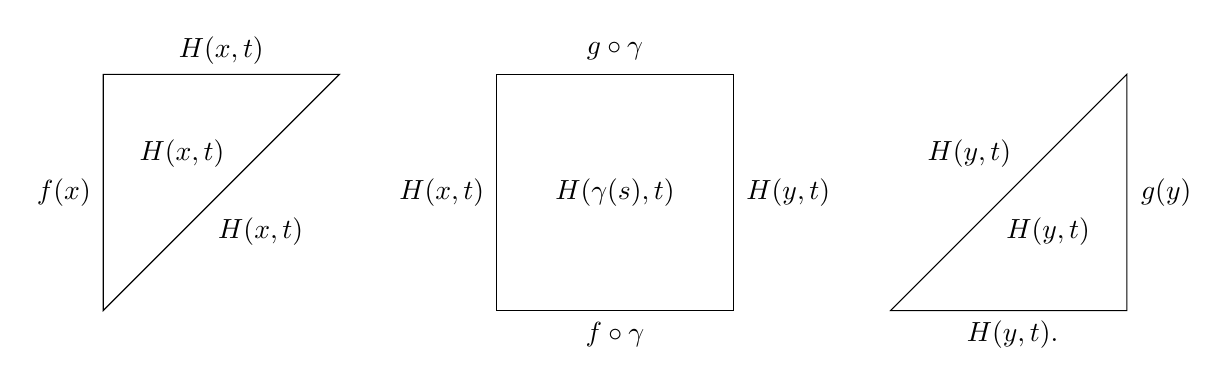
\begin{tikzpicture}[>=latex]
			\draw (0, 0) node {}
			-- (0, 3) node {}
			-- (3, 3) node {}
			-- cycle;
			\draw (1.5, 3.3) node {$H(x, t)$};
			\draw (-0.5, 1.5) node {$f(x)$};
			\draw (1.0, 2.0) node {$H(x, t)$};
			\draw (2.0, 1.0) node {$H(x, t)$};

			\draw (5,0) rectangle (8, 3);
			\draw (4.3, 1.5) node {$H(x, t)$};
			\draw (8.7, 1.5) node {$H(y, t)$};
			\draw (6.5, 1.5) node {$H(\gamma(s), t)$};
			\draw (6.5, 3.3) node {$g\circ\gamma$};
			\draw (6.5, -0.3) node {$f\circ\gamma$};

			\draw (13, 3) node {}
			-- (10, 0) node {}
			-- (13, 0) node {}
			-- cycle;
			\draw (11.5, -0.3) node {$H(y, t)$\punctuation{.}};
			\draw (13.5, 1.5) node {$g(y)$};
			\draw (11.0, 2.0) node {$H(y, t)$};
			\draw (12.0, 1.0) node {$H(y, t)$};
		\end{tikzpicture}
	\end{figure}
	This gives precisely the desired homotopy.
\end{proof}


\begin{thm}\label{homotopy invariance}
	Let $X\simeq Y$. Then $\Pi_1X\simeq \Pi_1Y$.
\end{thm}

\begin{proof}
	Let $f: X\rightarrow Y$ and $g: Y\rightarrow X$ be homotopy equivalences, so
	that $gf\simeq 1_X$ and $fg\simeq 1_Y$. The fundamental groupoid induces
	groupoid morphisms $$\Pi_1f: \Pi_1X\rightarrow\Pi_1Y\quad\text{and}\quad\Pi_1g:
		\Pi_1Y\rightarrow\Pi_1X.$$
	We show these form equivalences $\Pi_1X\simeq \Pi_1Y$. By the lemma, we have
	that $$\Pi_1g\Pi_1f = \Pi_1 gf\cong \Pi_1{1_X} = 1_{\Pi_1 X};$$ the other
	direction follows by symmetry of the situation.
\end{proof}

\section{2-Categories, Briefly}
\label{2 categories}

The analogy we've drawn between homotopies and natural transformation can be
made rigorous in several ways. Here we sketch maybe the easiest, and discuss its
limitations. The main objective is to generalize categories to allow morphisms
between morphisms, like homotopies in $\cat{Top}$ and natural transformations in
$\cat{Cat}$. I largely follow \cite[Chapter 1]{Leinster}.

Note that in an ordinary (locally small) category, the morphisms $\cat{C}(x, y)$
form a set for any pair of objects. In many settings, we can say something
stronger: recall, for instance, that the set of linear transformations $\cL(V,
	W)$ between any two vector spaces is itself a vector space. This is called
\emph{enrichment} over $\cat{Vect}_\Bbbk$.

We can't enrich with every category, at least not if we want the resultant
structure to be interesting. Say we want to enrich over the category $\cat{K}$.
Presumably, we want composition to capture the internal structure of $\cat{K}$.
The easiest way to ensure this is to ask that $\cat{K}$ have a kind of internal
product, which will allow us to define composition.

\begin{defn}
	A \emph{monoidal category} consists of a category $\cat{K}$, a functor
	$\otimes: \cat{K}\times\cat{K}\rightarrow\cat{K}$ called the \emph{tensor
		product}, an object $1_\otimes\in A$ called the \emph{tensor unit}, and natural
	isomorphisms
	$$\alpha_{x,y,z}: (x\otimes y)\otimes z\simeq x\otimes(y\otimes z),\quad
		\lambda_x: 1_\otimes\otimes x\simeq x,\quad \rho_x: x\otimes1_\otimes\simeq xm$$
	called the \emph{coherence isomorphisms}.

	This data must satisfy the \emph{triangle} and \emph{pentagon} identities:

	\begin{figure}[H]
		\centering
		\begin{tikzcd}
			(x\otimes 1_\otimes)\otimes y & & x\otimes(1_\otimes\otimes y) \\
			& x\otimes y &
			\arrow["\alpha_{x,1_\otimes,y}", from=1-1, to=1-3]
			\arrow["\rho_x", from=1-1, to=2-2, swap]
			\arrow["\lambda_x", from=1-3, to=2-2]
		\end{tikzcd}
		\begin{tikzcd}
			& (x\otimes y)\otimes(z\otimes w) & \\
			((x\otimes y)\otimes z)\otimes w & & x\otimes (y\otimes (z\otimes w)) \\
			(x\otimes (y\otimes z))\otimes w & & x\otimes ((y\otimes z)\otimes w)\punctuation{.}
			\arrow["\alpha_{x\otimes y, z, w}", from=2-1, to=1-2]
			\arrow["\alpha_{x, y, z\otimes w}", from=1-2, to=2-3]
			\arrow["\alpha_{x, y, z}\otimes 1_w", from=2-1, to=3-1, swap]
			\arrow["1_x\otimes\alpha_{y, z, w}", from=3-3, to=2-3, swap]
			\arrow["\alpha_{x, y\otimes z, w}", from=3-1, to=3-3, swap]
		\end{tikzcd}
	\end{figure}

	Asking for uniqueness (as opposed to isomorphism) of associates turns out to be
	too much, but these identities ask just that the composite coherence
	isomorphisms are unique.
\end{defn}

\begin{ex}
	One can check that $\cat{Vect}_\Bbbk$, $\cat{Set}$, and $\cat{Cat}$ each have
	monoidal structure, with the (vector space) tensor, the Cartesian product, and
	the product category, respectively. These examples show why we can only ask
	for isomorphism of identities and associates: the one-element set is not
	exactly its own Cartesian product, but it is isomorphic to it.
\end{ex}


\begin{defn}\label{enrichment}
	Let $\cat{K}$ be a monoidal category. A \emph{category enriched over
		$\cat{K}$}, $\cat{C}$, consists of
	\begin{itemize}
		\item A collection of objects.
		\item For each pair of objects $x,y$, an object $\cat{C}(x, y)$ in
		      $\cat{K}$.
		\item For each triple of objects $x,y,z$, a morphism $\circ_{x, y, z}\cat{C}(y,
			      z)\otimes\cat{C}(x, y)\rightarrow\cat{C}(x, z)$, called composition.
		\item For each object $x$, a morphism $1_x: 1_\otimes\rightarrow C(x, x)$, called the
		      identity morphism.
	\end{itemize}

	This data must satisfy certain \emph{associative} and \emph{unital} laws:

	\begin{figure}[H]
		\centering
		\begin{tikzcd}
			(\cat{C}(z, w)\otimes\cat{C}(y,z))\otimes\cat{C}(x, y)
			& & \cat{C}(z, w)\otimes(\cat{C}(y,z)\otimes\cat{C}(x, y)) \\
			\cat{C}(y, w)\otimes\cat{C}(x, y)
			& \cat{C}(x, y)
			& \cat{C}(z, w)\otimes(\cat{C}(x, z)) \\
			\arrow["\alpha_{\cat{C}(z, w),\cat{C}(y,z),\cat{C}(x, y)}", from=1-1, to=1-3]
			\arrow["\circ_{y, z, w}\otimes1_{\cat{C}(x, y)}", from=1-1, to=2-1, swap]
			\arrow["1_{\cat{C}(z, w)}\otimes\circ_{x, y, z}", from=1-3, to=2-3]
			\arrow["\circ_{x, y, w}", from=2-1, to=2-2, swap]
			\arrow["\circ_{x, z, w}", from=2-3, to=2-2]
		\end{tikzcd}
		\begin{tikzcd}
			\cat{C}(y, y)\otimes\cat{C}(x, y) & \cat{C}(x, y) & \cat{C}(x, y)\otimes\cat{C}(x, x) \\
			1_\otimes\otimes\cat{C}(x, y) & & \cat{C}(x, y)\otimes 1_\otimes
			\arrow["\circ_{x, y, y}", from=1-1, to=1-2]
			\arrow["\circ_{x, x, y}", from=1-3, to=1-2, swap]
			\arrow["1_y\otimes1_{\cat{C}(x, y)}", from=2-1, to=1-1]
			\arrow["\lambda_{C(x, y)}", from=2-1, to=1-2, swap]
			\arrow["\rho_{C(x, y)}", from=2-3, to=1-2]
			\arrow["1_{\cat{C}(x, y)}\times1_x", from=2-3, to=1-3, swap]
		\end{tikzcd}
	\end{figure}

	These laws guarantee that composites and identities work as expected.
\end{defn}

\begin{ex}We have two examples so far:
	\begin{itemize}
		\item A locally small category is a category enriched over $\cat{Set}$ (with
		      the Cartesian product).
		\item $\cat{Vect}_\Bbbk$ can be viewed as a category enriched over itself.
	\end{itemize}
\end{ex}

We can now define our main object:

\begin{defn}\label{2-category}	A \emph{strict 2-category} is\footnote{There is also an axiomatization of
		2-categories which requires less machinery and simply lists out all the axioms
		for 0-, 1-, and 2-cells deducible from \Cref{2-category}. See e.g. \cite[Section
			1.7]{Riehl}.} a category enriched over $\cat{Cat}$.
\end{defn}

\begin{ex}
	There is a 2-category of 1-categories, $\cat{1Cat}$, where the categorical
	structure on morphisms is given by vertical composition of natural
	transformations. In that case, horizontal composition gives exactly the right
	gadget to make the monoidal structure work.
\end{ex}

We can keep going:

\begin{defn} A \emph{0-category} is a set. An \emph{(n+1)-category} is a category
	enriched over $\cat{nCat}$, the category of all $n$-categories.
\end{defn}

To make the analogy between homotopies and natural transformations rigorous, we
would like to assemble spaces, continuous maps, and homotopies into a
2-category. However, we run into issues with associativity, since homotopies
only associate up to homotopy.

One way to fix associativity is to take homotopy classes of homotopies as our
2-cells. In fact, there is a strict 2-category of spaces, continuous functions,
and homotopy classes of homotopies. Many of the similarities between homotopy
and natural transformation we've observed can be studied in this setting. For
example, \Cref{two compositions} just observes that one has both the composite
morphisms and composition within the functor categories. In this setting
\Cref{pseudofunctor}, and its corollary \Cref{homotopy invariance}, have to do
with the \emph{weak 2-functoriality} of the fundamental groupoid.

This approach works for the case $n=2$, but it will break down quickly.
Informally, either our 3-cell structure will have to be trivial, since we would
be asking for homotopies between homotopy classes, or we will have to sacrifice
associativity for 2-cells and therefore no longer be a strict 3-category.
Instead, one can weaken the notion of n-category to obtain weak n-categories, in
which the associative and unital laws of \Cref{enrichment} are weakened up to,
for example, appropriate isomorphism of 2-cells. There are several ways to make
this precise, which we won't sketch; see \cite{Leinster}.


\bibliographystyle{alpha}
\bibliography{references}

\end{document}
\end{document}


\bibliographystyle{alpha}
\bibliography{references}

\end{document}
\end{document}
